%=================================================================
% Modèle de devoir - Version française
% Auteur : <Votre nom>
% Description : Modèle LaTeX pour soumissions de devoirs
%=================================================================

\documentclass[12.0 pt,a4paper]{article}

 
%---------------------------------------------------------------
% PACKAGES
%---------------------------------------------------------------
\usepackage[T1]{fontenc}              % Encodage correct
\usepackage[utf8]{inputenc}           % Support UTF-8
\usepackage[french]{babel}            % Langue française
\usepackage{geometry}                 % Marges
\geometry{margin=2.0cm}
\usepackage{ amssymb }
\usepackage{amsmath,amssymb,amsthm}   % Math
\usepackage{graphicx}                 % Images
\usepackage{array}                    % Tableaux avancés
\usepackage{tikz}                     % K-maps, circuits logiques
\usetikzlibrary{matrix, positioning, automata, positioning, arrows.meta}  % Bibliothèques TikZ nécessaires

\usepackage{caption}                  % Légendes personnalisées
\usepackage{multirow}                 % Cellules multi-lignes
\usepackage{xcolor}                   % Couleurs
\usepackage{fancyhdr}                 % En-têtes / pieds de page

\usepackage{pdfpages}

\usepackage{import}
\usepackage{hyperref}                 % Liens hypertextes
\usepackage{float}                    % Placement précis
\usepackage{datetime}                 % Formatage de dates
\usetikzlibrary{calc}
\usepackage{tabu}
\usetikzlibrary{shapes, arrows, positioning}
\usepackage{changepage} % allows local margin changes
\usepackage{subfigure}
%---------------------------------------------------------------
% INFORMATIONS DU COURS ET DU GROUPE
%---------------------------------------------------------------
\newcommand{\codeclasse}{ELE140}                     % Code du cours
\newcommand{\nomclasse}{Conception des systèmes numériques} % Nom du cours
\newcommand{\titredevoir}{Laboratoire 2} % Titre du devoir
\newcommand{\groupe}{-01}
\newcommand{\enseignant}{Myiah Catwell}
\newcommand{\datedepot}{\today}
\newcommand{\Session}{A25}
\newcommand{\auteurs}{
	Ourania Voyatzis~(VOYO78260401)\\
	Jhermain Louis-Jean~(LOUJ67360401)}

%---------------------------------------------------------------
% MISE EN PAGE
%---------------------------------------------------------------
\pagestyle{fancy}
\fancyhead[L]{\codeclasse\groupe}
\fancyhead[C]{\titredevoir}
\fancyhead[R]{\thepage}
\fancyfoot{}

%---------------------------------------------------------------
% DÉBUT DU DOCUMENT
%---------------------------------------------------------------
\begin{document}
	\section*{Q.1 a)}
\subsection*{Assignement des Bascules: "simplest"}
\begin{figure}[H]
\centering{\begin{tabular}{|c|c|}
	\hline
	INIT & 000 \\
	\hline
	X1 & 001 \\
	\hline
	X2 & 010 \\
	\hline
	X3 & 011 \\
	\hline
	X4 & 100 \\
	\hline
	OK & 101 \\
	\hline
\end{tabular}}
\end{figure}

\subsection*{Diagramme d'états}
\begin{figure}[H]
	\centering
	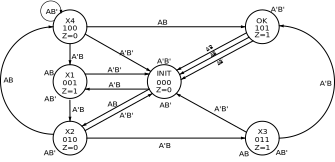
\includegraphics[width=0.7\linewidth]{BRUH}
	\caption{}
	\label{fig:bruh}
\end{figure}
\subsection*{Table de transitions}
\begin{figure}[H]
	\centering{\begin{tabular}{|c|c|c|c|c|c|}
			\hline
			\rule[-1ex]{0pt}{2.5ex}  & \multicolumn{4}{c|}{AB} & Z \\
			\hline
			\rule[-1ex]{0pt}{2.5ex} Q2,Q1,Q0 & 00 & 01 & 11 & 10 &  \\
			\hline
			\rule[-1ex]{0pt}{2.5ex} 000 & 000 & 001 & 010 & 000 & 0 \\
			\hline
			\rule[-1ex]{0pt}{2.5ex} 001 & 000 & 010 & 001 & 001 & 1 \\
			\hline
			\rule[-1ex]{0pt}{2.5ex} 010 & 000 & 011 & 100 & 010 & 0 \\
			\hline
			\rule[-1ex]{0pt}{2.5ex} 011 & 000 & 101 & 011 & 011 & 1 \\
			\hline
			\rule[-1ex]{0pt}{2.5ex} 100 & 000 & 001 & 101 & 100 & 0 \\
			\hline
			\rule[-1ex]{0pt}{2.5ex} 101 & 101 & 000 & 000 & 000 & 1 \\
			\hline
			\rule[-1ex]{0pt}{2.5ex}  & \multicolumn{4}{c|}{Q2*Q1*Q0*} &  \\
			\hline
	\end{tabular}}
\end{figure}

\section*{Tables de Karnaugh des Bascules (Combinatoire)}

\begin{figure}[H]
	\centering
		\subsection*{Q2*} % use subsection* to avoid numbering
	\begin{tikzpicture}
	\matrix (m) [matrix of nodes,
	nodes={draw, minimum size=1.2cm, anchor=center},
	column sep=-\pgflinewidth, row sep=-\pgflinewidth] {
		0 & 0 & 0 & 0 & X & X & 1 & 0 \\
		0 & 0 & 1 & 0 & X & X & 0 & 0 \\
		0 & 0 & 0 & 1 & X & X & 0 & 1 \\
		0 & 0 & 0 & 0 & X & X & 0 & 1 \\
	};
	\footnotesize
	\node[above=4pt of m-1-1] {$\overline{Q_2}\overline{Q_1}\overline{Q_0}$};
	\node[above=4pt of m-1-2] {$\overline{Q_2}\overline{Q_1}Q_0$};
	\node[above=4pt of m-1-3] {$\overline{Q_2}Q_1Q_0$};
	\node[above=4pt of m-1-4] {$\overline{Q_2}Q_1\overline{Q_0}$};
	\node[above=4pt of m-1-5] {$Q_2Q_1\overline{Q_0}$};
	\node[above=4pt of m-1-6] {$Q_2Q_1Q_0$};
	\node[above=4pt of m-1-7] {$Q_2\overline{Q_1}Q_0$};
	\node[above=4pt of m-1-8] {$Q_2\overline{Q_1}Q_0$};
	
	\node[left=4pt of m-1-1, rotate=90, anchor=south] {$\overline{A}\overline{B}$};
	\node[left=4pt of m-2-1, rotate=90, anchor=south] {$\overline{A}B$};
	\node[left=4pt of m-3-1, rotate=90, anchor=south] {$AB$};
	\node[left=4pt of m-4-1, rotate=90, anchor=south] {$A\overline{B}$};
\end{tikzpicture}
\caption{$Q2^*(A, B, Q2, Q1, Q0) = A'B'Q2Q0 + A'BQ1Q0 + AQ2Q0' + ABQ1Q0'$}


		\subsection*{Q1*}
	\begin{tikzpicture}
	\matrix (m) [matrix of nodes,
	nodes={draw, minimum size=1.2cm, anchor=center},
	column sep=-\pgflinewidth, row sep=-\pgflinewidth] {
		0 & 0 & 0 & 0 & X & X & 0 & 0 \\
		0 & 1 & 0 & 1 & X & X & 0 & 0 \\
		1 & 0 & 1 & 0 & X & X & 0 & 0 \\
		0 & 0 & 1 & 1 & X & X & 0 & 0 \\
	};
	\footnotesize
	\node[above=4pt of m-1-1] {$\overline{Q_2}\overline{Q_1}\overline{Q_0}$};
	\node[above=4pt of m-1-2] {$\overline{Q_2}\overline{Q_1}Q_0$};
	\node[above=4pt of m-1-3] {$\overline{Q_2}Q_1Q_0$};
	\node[above=4pt of m-1-4] {$\overline{Q_2}Q_1\overline{Q_0}$};
	\node[above=4pt of m-1-5] {$Q_2Q_1\overline{Q_0}$};
	\node[above=4pt of m-1-6] {$Q_2Q_1Q_0$};
	\node[above=4pt of m-1-7] {$Q_2\overline{Q_1}Q_0$};
	\node[above=4pt of m-1-8] {$Q_2\overline{Q_1}Q_0$};
	
	\node[left=4pt of m-1-1, rotate=90, anchor=south] {$\overline{A}\overline{B}$};
	\node[left=4pt of m-2-1, rotate=90, anchor=south] {$\overline{A}B$};
	\node[left=4pt of m-3-1, rotate=90, anchor=south] {$AB$};
	\node[left=4pt of m-4-1, rotate=90, anchor=south] {$A\overline{B}$};
\end{tikzpicture}
\caption{$Q1^*(A, B, Q2, Q1, Q0) = A'BQ2'Q1'Q0 + A'BQ1Q0' + AB'Q1 + ABQ2'Q1'Q0' + AQ1Q0$}
	\subsection*{Q0*}
	\begin{tikzpicture}
		\matrix (m) [matrix of nodes,
		nodes={draw, minimum size=1.2cm, anchor=center},
		column sep=-\pgflinewidth, row sep=-\pgflinewidth] {
			0 & 0 & 0 & 0 & X & X & 1 & 0 \\
			1 & 0 & 1 & 1 & X & X & 0 & 1 \\
			0 & 1 & 1 & 0 & X & X & 0 & 1 \\
			0 & 1 & 1 & 0 & X & X & 0 & 0 \\
		};
	\footnotesize
		\node[above=4pt of m-1-1] {$\overline{Q_2}\overline{Q_1}\overline{Q_0}$};
		\node[above=4pt of m-1-2] {$\overline{Q_2}\overline{Q_1}Q_0$};
		\node[above=4pt of m-1-3] {$\overline{Q_2}Q_1Q_0$};
		\node[above=4pt of m-1-4] {$\overline{Q_2}Q_1\overline{Q_0}$};
		\node[above=4pt of m-1-5] {$Q_2Q_1\overline{Q_0}$};
		\node[above=4pt of m-1-6] {$Q_2Q_1Q_0$};
		\node[above=4pt of m-1-7] {$Q_2\overline{Q_1}Q_0$};
		\node[above=4pt of m-1-8] {$Q_2\overline{Q_1}Q_0$};
		
		\node[left=4pt of m-1-1, rotate=90, anchor=south] {$\overline{A}\overline{B}$};
		\node[left=4pt of m-2-1, rotate=90, anchor=south] {$\overline{A}B$};
		\node[left=4pt of m-3-1, rotate=90, anchor=south] {$AB$};
		\node[left=4pt of m-4-1, rotate=90, anchor=south] {$A\overline{B}$};
	\end{tikzpicture}
	\caption{$Q0^*(A, B, Q2, Q1, Q0) = A'B'Q2Q0 + A'BQ0' + AQ2'Q0 + BQ2Q0' + A'BQ1$}
\end{figure}
\section*{Q1 b)}
\subsection*{Table de transitions}
\begin{figure}[H]
	\centering{\begin{tabular}{|c|c|c|c|c|c|}
			\hline
			\rule[-1ex]{0pt}{2.5ex}  & \multicolumn{4}{c|}{AB} & Z \\
			\hline
			\rule[-1ex]{0pt}{2.5ex} Q2 Q1 Q0 & 00 & 01 & 11 & 10 &  \\
			\hline
			\rule[-1ex]{0pt}{2.5ex} 111 & 111 & 110 & 010 & 111 & 0 \\
			\hline
			\rule[-1ex]{0pt}{2.5ex} 011 & 111 & 010 & 011 & 011 & 1 \\
			\hline
			\rule[-1ex]{0pt}{2.5ex} 010 & 111 & 001 & 000 & 010 & 0 \\
			\hline
			\rule[-1ex]{0pt}{2.5ex} 001 & 111 & 100 & 001 & 001 & 1 \\
			\hline
			\rule[-1ex]{0pt}{2.5ex} 000 & 111 & 011 & 100 & 000 & 0 \\
			\hline
			\rule[-1ex]{0pt}{2.5ex} 100 & 100 & 111 & 111 & 111 & 1 \\
			\hline
			\rule[-1ex]{0pt}{2.5ex}  & \multicolumn{4}{c|}{Q2*Q1*Q0*} &  \\
			\hline
	\end{tabular}}
\end{figure}

\subsection*{Tables de Karnaugh des Bascules (Combinatoire) b)}
\paragraph*{}
Dans les états indéfinis (001,101), nous revenons à l'état initial (tout à 1) afin de minimiser les risques.
\begin{figure}[H]
	\centering
	\subsection*{Q2*} % use subsection* to avoid numbering
	\begin{tikzpicture}
		\matrix (m) [matrix of nodes,
		nodes={draw, minimum size=1.2cm, anchor=center},
		column sep=-\pgflinewidth, row sep=-\pgflinewidth] {
			1 & 1 & 1 & 1 & 1 & 1 & 1 & 1 \\
			0 & 1 & 0 & 0 & 1 & 1 & 1 & 1 \\
			1 & 0 & 0 & 0 & 1 & 0 & 1 & 1 \\
			0 & 0 & 0 & 0 & 1 & 1 & 1 & 1 \\
		};
		\footnotesize
		\node[above=4pt of m-1-1] {$\overline{Q_2}\overline{Q_1}\overline{Q_0}$};
		\node[above=4pt of m-1-2] {$\overline{Q_2}\overline{Q_1}Q_0$};
		\node[above=4pt of m-1-3] {$\overline{Q_2}Q_1Q_0$};
		\node[above=4pt of m-1-4] {$\overline{Q_2}Q_1\overline{Q_0}$};
		\node[above=4pt of m-1-5] {$Q_2Q_1\overline{Q_0}$};
		\node[above=4pt of m-1-6] {$Q_2Q_1Q_0$};
		\node[above=4pt of m-1-7] {$Q_2\overline{Q_1}Q_0$};
		\node[above=4pt of m-1-8] {$Q_2\overline{Q_1}Q_0$};
		
		\node[left=4pt of m-1-1, rotate=90, anchor=south] {$\overline{A}\overline{B}$};
		\node[left=4pt of m-2-1, rotate=90, anchor=south] {$\overline{A}B$};
		\node[left=4pt of m-3-1, rotate=90, anchor=south] {$AB$};
		\node[left=4pt of m-4-1, rotate=90, anchor=south] {$A\overline{B}$};
	\end{tikzpicture}
	\caption{$Q2^*(A, B, Q2, Q1, Q0) = A'B' + A'Q1'Q0 + A'Q2 + B'Q2 + ABQ1'Q0' + Q2Q1' + Q2Q0'$}
\end{figure}
	
	\begin{figure}[H]
		\centering
	\subsection*{Q1*}

	\begin{tikzpicture}
		\matrix (m) [matrix of nodes,
		nodes={draw, minimum size=1.2cm, anchor=center},
		column sep=-\pgflinewidth, row sep=-\pgflinewidth] {
			1 & 1 & 1 & 1 & 1 & 1 & 1 & 0 \\
			1 & 0 & 1 & 0 & 1 & 1 & 1 & 1 \\
			0 & 0 & 1 & 0 & 1 & 1 & 1 & 1 \\
			0 & 0 & 1 & 1 & 1 & 1 & 1 & 1 \\
		};
		\footnotesize
		\node[above=4pt of m-1-1] {$\overline{Q_2}\overline{Q_1}\overline{Q_0}$};
		\node[above=4pt of m-1-2] {$\overline{Q_2}\overline{Q_1}Q_0$};
		\node[above=4pt of m-1-3] {$\overline{Q_2}Q_1Q_0$};
		\node[above=4pt of m-1-4] {$\overline{Q_2}Q_1\overline{Q_0}$};
		\node[above=4pt of m-1-5] {$Q_2Q_1\overline{Q_0}$};
		\node[above=4pt of m-1-6] {$Q_2Q_1Q_0$};
		\node[above=4pt of m-1-7] {$Q_2\overline{Q_1}Q_0$};
		\node[above=4pt of m-1-8] {$Q_2\overline{Q_1}Q_0$};
		
		\node[left=4pt of m-1-1, rotate=90, anchor=south] {$\overline{A}\overline{B}$};
		\node[left=4pt of m-2-1, rotate=90, anchor=south] {$\overline{A}B$};
		\node[left=4pt of m-3-1, rotate=90, anchor=south] {$AB$};
		\node[left=4pt of m-4-1, rotate=90, anchor=south] {$A\overline{B}$};
	\end{tikzpicture}
	\caption{$Q1^*(A, B, Q2, Q1, Q0) = Q1Q0 + B'Q1 + AQ2 + A'Q2'Q1'Q0' + A'B'Q0 + BQ2$}
\end{figure}
		\begin{figure}[H]
		\centering
	\subsection*{Q0*}

	\begin{tikzpicture}
		\matrix (m) [matrix of nodes,
		nodes={draw, minimum size=1.2cm, anchor=center},
		column sep=-\pgflinewidth, row sep=-\pgflinewidth] {
			1 & 1 & 1 & 1 & 1 & 1 & 1 & 0 \\
			1 & 0 & 0 & 1 & 1 & 0 & 1 & 1 \\
			0 & 1 & 1 & 0 & 1 & 0 & 1 & 1 \\
			0 & 1 & 1 & 0 & 1 & 1 & 1 & 1 \\
		};
		\footnotesize
		\node[above=4pt of m-1-1] {$\overline{Q_2}\overline{Q_1}\overline{Q_0}$};
		\node[above=4pt of m-1-2] {$\overline{Q_2}\overline{Q_1}Q_0$};
		\node[above=4pt of m-1-3] {$\overline{Q_2}Q_1Q_0$};
		\node[above=4pt of m-1-4] {$\overline{Q_2}Q_1\overline{Q_0}$};
		\node[above=4pt of m-1-5] {$Q_2Q_1\overline{Q_0}$};
		\node[above=4pt of m-1-6] {$Q_2Q_1Q_0$};
		\node[above=4pt of m-1-7] {$Q_2\overline{Q_1}Q_0$};
		\node[above=4pt of m-1-8] {$Q_2\overline{Q_1}Q_0$};
		
		\node[left=4pt of m-1-1, rotate=90, anchor=south] {$\overline{A}\overline{B}$};
		\node[left=4pt of m-2-1, rotate=90, anchor=south] {$\overline{A}B$};
		\node[left=4pt of m-3-1, rotate=90, anchor=south] {$AB$};
		\node[left=4pt of m-4-1, rotate=90, anchor=south] {$A\overline{B}$};
	\end{tikzpicture}
	\caption{$Q0^*(A, B, Q2, Q1, Q0) = AQ2'Q0 + A'B'Q2' + Q2Q1'Q0 + B'Q2Q1 + A'BQ0' + AQ2Q0'$}
\end{figure}



\end{document}